
\section{Signal Model}

\begin{figure}[htbp]
	\centering
	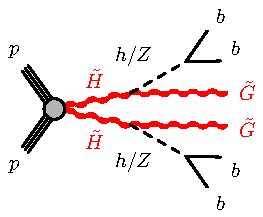
\includegraphics[width=0.35\textwidth]{figures/ewk_prod/varie/N1N1-hhGG-bbbb_Z}
	\caption{Diagram for the simplified model considered in the analysis. The primary interpretation of the analysis is the decay via Higgs bosons, but decays via varied branching ratios to $Z$ bosons are also studied. The production of the \hino\ occurs
via mass-degenerate pairs of charginos or neutralinos, which decay to the \ninoone\ and immeasurably low momentum particles.} 
	\label{fig:feyn}
\end{figure}

\subsection{Signal cross section}

%\section{Previous Limits}

